%
% Another appendix chapter
\chapter{Constrained Orbital Energy Trajectories}
[GEBRUIK LIMITS IN ALPHA EN LEG UIT OF GRADIENT NIET KAN] The inputs of height acceleration or inputs along the virtual leg have a changing effect proportional to the distance from the point foot. Next to this, if the goal of capture is considered, there exist a predetermined final point in the resulting trajectory of the control law. Namely, where the point-mass is above the point-foot, or the instable equilibrium of the inverted pendulum. With a simple proportial control law, no effects forward in time would be known. To have knowledge of the state variables of the model forward in time, the \ac{LIP} orbital energy, discussed in \ref{subsec:liporbit}, was extended by a height varying version by writing the height as a function of the horizontal position in  \cite{pratt2007derivation}, as mentioned in \ref{subsec:nonorbit}. This extra bit of information can be used in different ways, as for example in replanning the dynamic plan, or in \ac{MPC}. Depending on the way a dynamic plan is generated, the distinctionb between \ac{MPC} and dynamic replanning can be very small. In this chapter, the \ac{MPC} from \cite{koolen2016balance} is extended with constraints, which can be used for either dynamic replanning or \ac{MPC}.

%% Constraint matrix/polynomial
\section{Constraint Matrix}
In \cite{koolen2016balance}, the final horizontal velocity $\dot{x}_f$ is set to zero, as this leads to a capture trajectory. However, the trajectories are unconstrained and can become unrealistically high, as shown in \figref{fig:cpbal}. If from the final velocity is left open from the nonlinear orbital energy, this can be used in constrained optimization. A recap of Equation \ref{eq:eorbit}, but setting the final horizontal position zero:
\begin{equation}
    \frac{1}{2}\dot{x}^2\bar{f}^2(x)+gx^2f(x) - 3g\int_{0}^xf(\xi)\xi d\xi = \frac{1}{2}\dot{x}_0^2\bar{f}^2(0).
\end{equation}
Note that $\bar{f}^2(0)=(f(0)-f'(0)*0)^2=f(0)^2$. The additional nonzero term on the right side of the orbital energy equation can be added in the constraint matrix of \cite{koolen2016balance}. The 4x4 constraint matrix reads as:
\begin{equation}
    \underbrace{\begin{bmatrix}1 & 0 & 0 & 0 \\ 
     1 & x_0 & x_0^2 & x_0^3\\
     0 & 1 & 2x_0 & 3x_0^2\\
     \frac{3}{2}gx_0^2 & gx_0^3 & \frac{3}{4}gx_0^4 & \frac{3}{5}gx_0^5\\
     \end{bmatrix}}_{\matr{A}}
     \underbrace{\begin{bmatrix}
     c_0\\
     c_1\\
     c_2\\
     c_3\\
     \end{bmatrix}}_{\vect{c}}=
     \underbrace{\begin{bmatrix}
     z_f\\
     z_0\\
     \frac{\dot{z}_0}{\dot{x}_0}\\
     k\\
     \end{bmatrix}}_{\vect{b}}.
\end{equation}
Recap that the function $f(x)$ is constrained to be a cubic polynomial: $f(x)=\sum_{i=0}^3 c_ix^i$. The last constraint in the matrix is the constraint on conservation of orbital energy. Note that the integal term in the orbital energy equation read as: $3g\int_{0}^xf(\xi)\xi d\xi = 3g\sum_{i=0}^3\frac{1}{i+2}c_ix_0^{i+2}$. The last constraint of the matrix reads after addition of the final velocity term as:
\begin{equation}
		3g\int_{0}^xf(\xi)\xi d\xi =\frac{1}{2}\dot{x}^2\bar{f}^2(x)+gx^2f(x) - \frac{1}{2}\dot{x}_0^2\bar{f}^2(0),
\end{equation}
and in terms of the cubic polynomial as:
\begin{align}
	3g\sum_{i=0}^3\frac{1}{i+2}c_ix_0^{i+2}& = \frac{1}{2}(\dot{x}_0z_0-\dot{x}_0x_0)^2 + gx_0^2z_0 - \frac{1}{2}z_f^2\dot{x}_f^2,\\
	&=k,
\end{align}
where $k$ is the last value in vector $\vect{b}$. Using the polynomial description and having a nonzero final velocity $\dot{x}_f$, the final height $z_f$ constraint results in a final height velocity $\dot{z}_f$ equal to the gradient:
\begin{align}
 	f'(0) &= \frac{\dot{z}_f}{\dot{x}_f},\\
 	\dot{z}_f &= f'(0)\dot{x}_f.
\end{align}
If a nonzero final velocity $\dot{x}_f$ is considered, the pendulum is at the point $x=0$ at a point during swing. It could be desirable later, to have zero height velocity $\dot{z}_f$ at this point. The first constraint $f(0)=z_f$ in the matrix can be replaced by this constraint on this final gradient:
\begin{equation}
    \underbrace{\begin{bmatrix}0 & 1 & 0 & 0 \\ 
     1 & x_0 & x_0^2 & x_0^3\\
     0 & 1 & 2x_0 & 3x_0^2\\
     \frac{3}{2}gx_0^2 & gx_0^3 & \frac{3}{4}gx_0^4 & \frac{3}{5}gx_0^5\\
     \end{bmatrix}}_{\matr{A}}
     \underbrace{\begin{bmatrix}
     c_0\\
     c_1\\
     c_2\\
     c_3\\
     \end{bmatrix}}_{\vect{c}}=
     \underbrace{\begin{bmatrix}
    \frac{\dot{z}_f}{\dot{x}_f}\\
     z_0\\
     \frac{\dot{z}_0}{\dot{x}_0}\\
     k\\
     \end{bmatrix}}_{\vect{b}}
\end{equation}
Note that the matrix is still full rank, as long as $x_f$ and $\dot{x}_f$ are nonzero.
%\begin{equation}
%    u = \frac{g + f''(x)\dot{x}^2}{\bar{f}(x)}
%\end{equation}

% Height Constraint
\subsection{Height Constraint}
Using the previous problem with an undetermined final velocity $\dot{x}_f$, a height constraint can be used in optimization. Algorithm \ref{alg:h} shows how the polynomial values can be found under this constraint. The maximum height of trajectory being optimized over is at location $x_{zmax}$, which has two solutions. In \figref{fig:polheight} two resulting polynomials are shown from Algorithm \ref{alg:h}, one with the final height constraint and one for the constraint on the final gradient. Notice that the peak for the maximum value in both plots lies on the maximum $x$-value from the solutions of the locations where the gradient as zero. Therefore, in Algorithm \ref{alg:h} the solution that corresponds to this peak is sufficient, if a constraint on the maximum value is considered. In the plot of the figure, the entire polynomial is shown for explanatory reasons, but in control or planning only the part would be used from the starting point $x=-0.25$.
\begin{equation}
	\dot{x}_{f,cp} = \sqrt{\dot{x}_0^2-\frac{g}{z}x^2}
\end{equation}
\begin{equation}
	\dot{x}_{f,cp,maxheight} = \sqrt{\dot{x}_{0,I}^2-\frac{g}{z}(x+\frac{\dot{z}_I}{g}\dot{x}_{0,I})^2}
\end{equation}
\begin{equation}
	\alpha =\frac{\dot{x}_{f,cp} -\dot{x}_{f,cp,maxheight}}{N}
\end{equation}
$N=30$.

\begin{algorithm}
\caption{Find cubic polynomial constants under height constraint}
\label{alg:h}
\begin{algorithmic}[1]
    \State $\dot{x}_{f}\gets 0$\Comment{Initial guess}
        \Repeat
            \State $\vect{c}\gets \matr{A}^{-1}\vect{b}(\dot{x}_{f})$ \Comment{Find polynomial constants}
            \State $x_{zmax}\gets \frac{-2c_2 - \sqrt{4c_2^2-12c_3c_1}}{6c_3}$ \Comment{Traj. peak lies on highest x}
            \State $z_{max} \gets c_0 + c_1x_{zmax} + c_2x_{zmax}^2+ c_3x_{zmax}^3$ \Comment{Corresponding height}
            \State $\dot{x}_{f} \gets \dot{x}_{f}+\alpha$   \Comment{Some smart increment}
        \Until{$z_{max}<z_{const}$}\\
    \Return $\vect{c}$
\end{algorithmic}
\end{algorithm}
\begin{figure}[h]
\centering
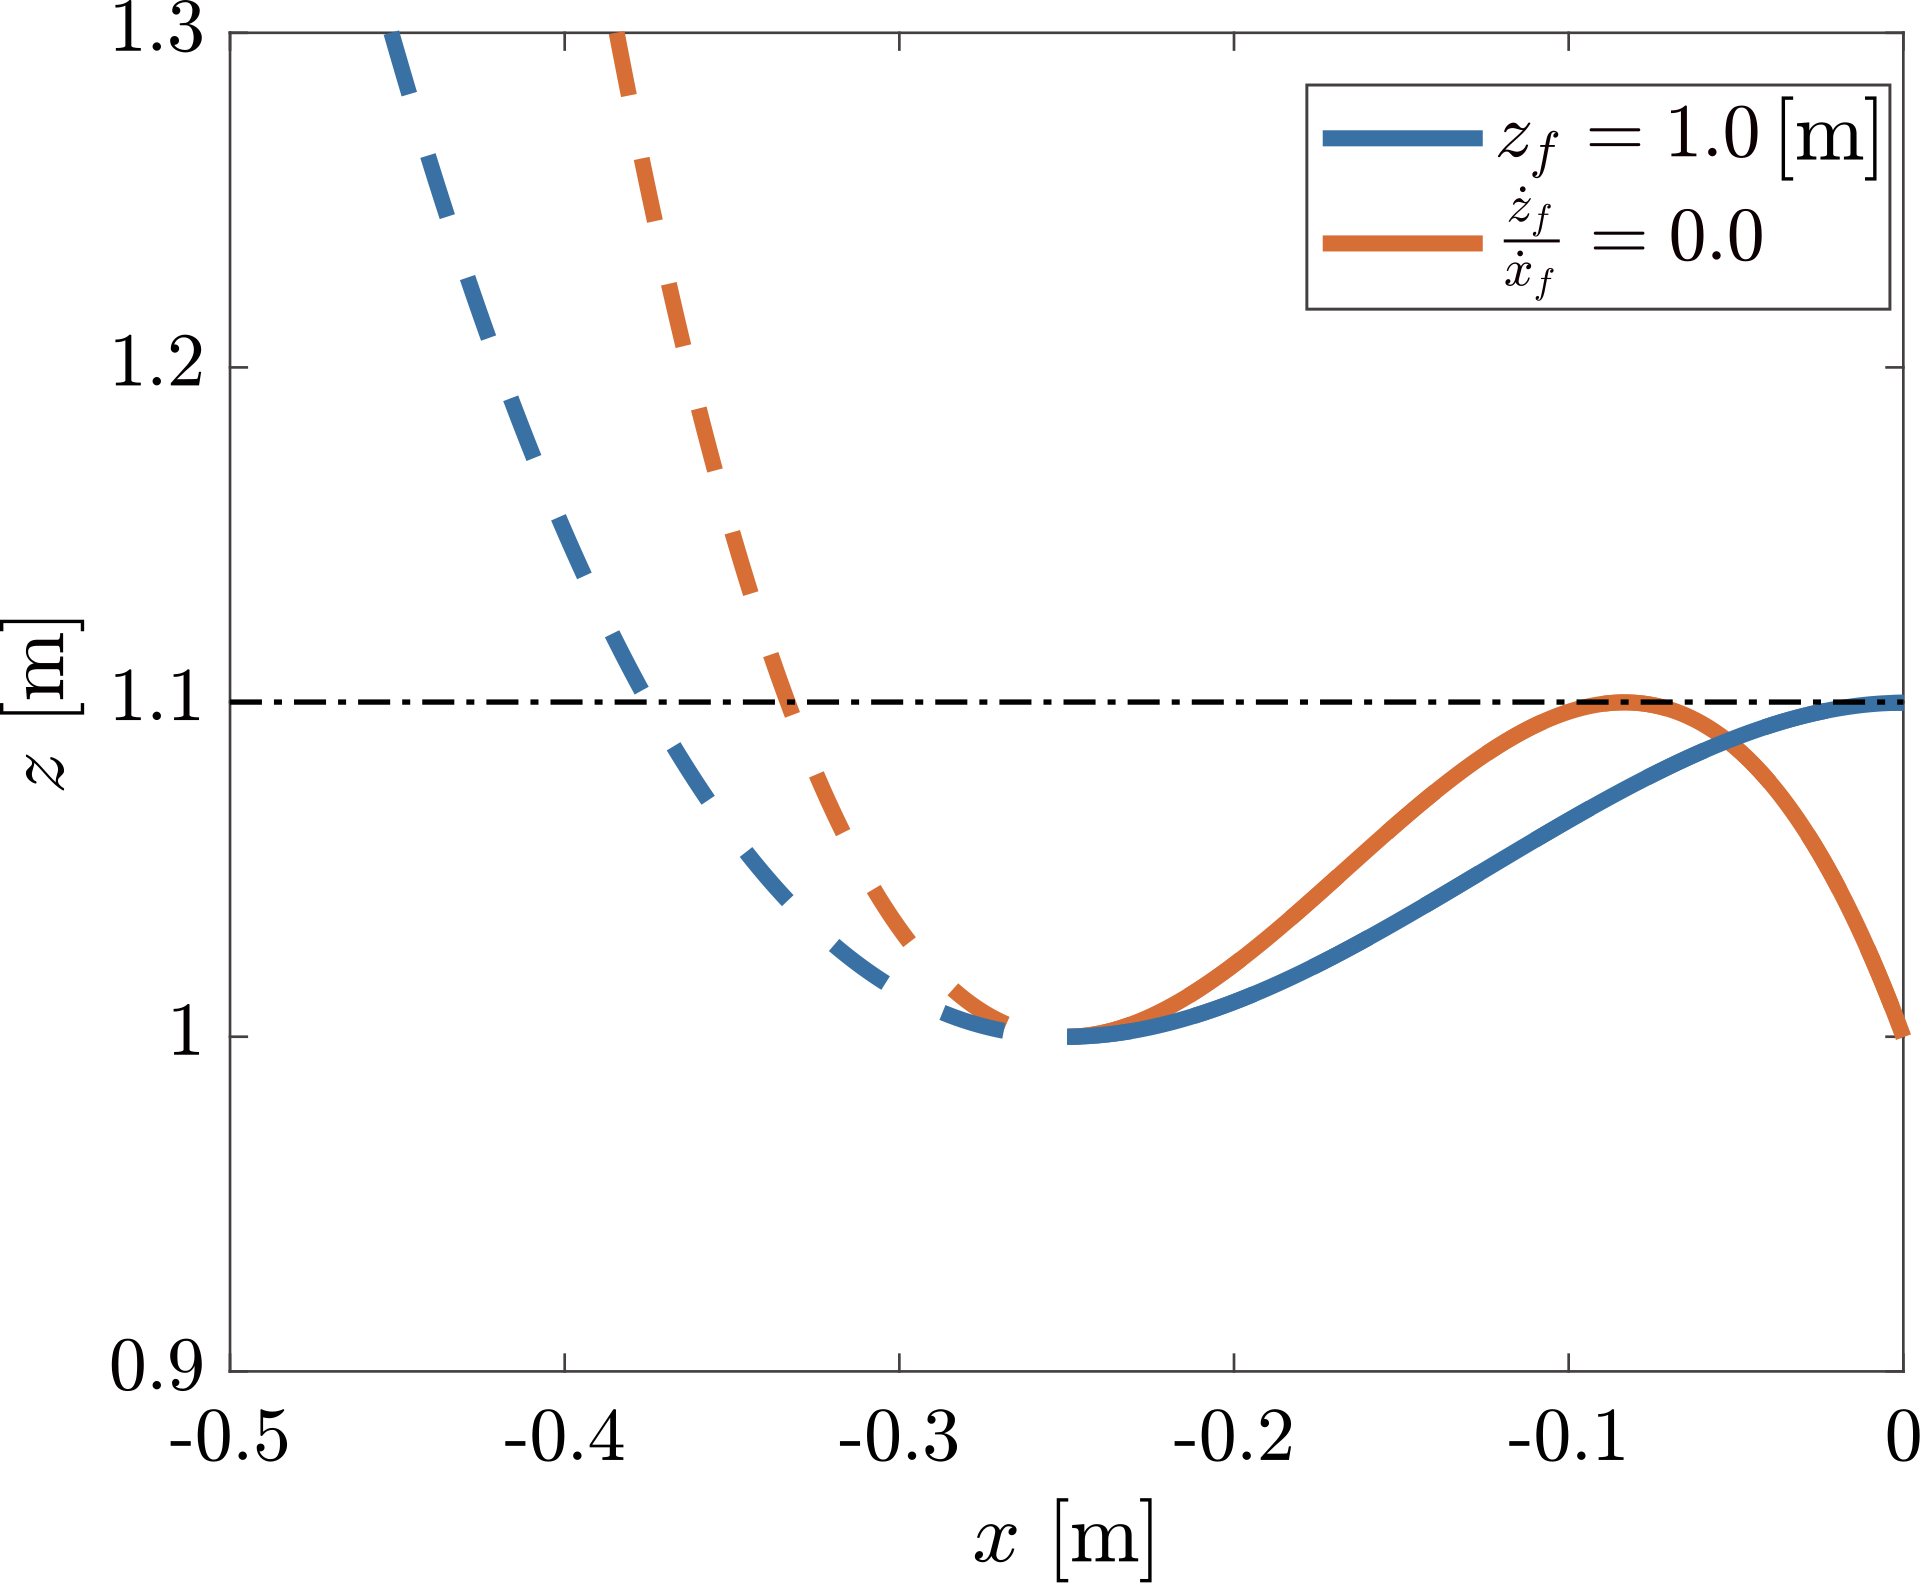
\includegraphics[width=0.6\textwidth]{STYLESTUFF/polynomialHeightViz.png}
\caption{Resulting polynomials as output from Algorithm \ref{alg:h} with two different constraints on the final value. Initial conditions are $x_0=-0.25$, $\dot{x}_0=1.0$, $z_0=1.0$ and $\dot{z}_0=0$. Blue plot: $\dot{x}_f=0.552$, red plot: $\dot{x}_f=0.576$, $z_{max}=1.1$. }
\label{fig:polheight}
\end{figure}


% leg length constraint
\subsection{Leg Length Constraint}
For application, a leg e length constraint would be more realistic than a height constraint. The leg length as a function of $x$ can be expressed using the Pythagorean theorem:
\begin{equation}
	l^2(x) = f(x)^2 + x^2,
\end{equation}
where $l$ the length of the virtual leg. The solution to $f(x)^2$ is:
\begin{equation}
f(x)^2=(\sum_{n=0}^3 c_n x^n)^2 = \sum_{n=0}^3 c_n^2 x^{2n} + 2\sum_{\substack{n=1 \\ i+j=n \\ i < j}}^5 c_i c_j x^n. 
\end{equation}
However, as the gradient needs to be computed to obtain the locations of the peaks in the polynomial, $f(x)^2$ is approximated with:
\begin{equation*}
	f(x)^2\approx \sum_{n=0}^3 c_n^2 x^{2n}.
\end{equation*}
With this formulation of the squared function, the squared $x$ position of maximum leg length is computed in the following way:
\begin{align}
	\frac{d(f(x)^2+x^2)}{dx}&=0\\
	\frac{d(f(x)^2+x^2)x}{dx}&=0\\
	6c_3^2 x^4 + 4 c_2^2 x^2 + 2+2c_1^2 &= 0\\
	6c_3^2 (x^2)^2 + 4 c_2^2 (x^2) + 2+2c_1^2 &= 0
\end{align}
Again, the value of the maximum peak lies on the highest $x$ value of the two locations where the gradient is zero. Algorithm \ref{alg:ll} shows how the polynomial constants can be found under the leg length constraint. In Figure \ref{fig:pollength}, it can be seen that the resulting polynomials do not violate the maximum length constraint.
\begin{algorithm}
\caption{Find cubic polynomial constants under leg length constraint}
\label{alg:ll}
\begin{algorithmic}[1]
    \State $\dot{x}_{f}\gets 0$\Comment{Initial guess}
        \Repeat
            \State $\vect{c}\gets \matr{A}^{-1}\vect{b}(\dot{x}_{f})$ \Comment{Find polynomial constants}
            \State $x_{lmax}^2 \gets \frac{-4c_2^2+\sqrt{16c_2^4-24c_3^2(2+2c_1^2)}}{12c_3^2}$ \Comment{$d(f(x)^2+x^2)/dx=0$}  
            \State $x_{lmax}\gets-|\sqrt{x_{l^2max}}|$                \Comment{Complex solutions}
            \State $l_{max}^2 \gets x_{lmax}^2 + (c_0 + c_1x_{zmax} + c_2x_{zmax}^2+ c_3x_{zmax}^3)^2$ 
            \State $\dot{x}_{f} \gets \dot{x}_{f}+\alpha$   \Comment{Some smart increment}
        \Until{$l_{max}^2<l_{const}^2$}\\
    \Return $\vect{c}$    
\end{algorithmic}
\end{algorithm}
\begin{figure}[h]
\centering
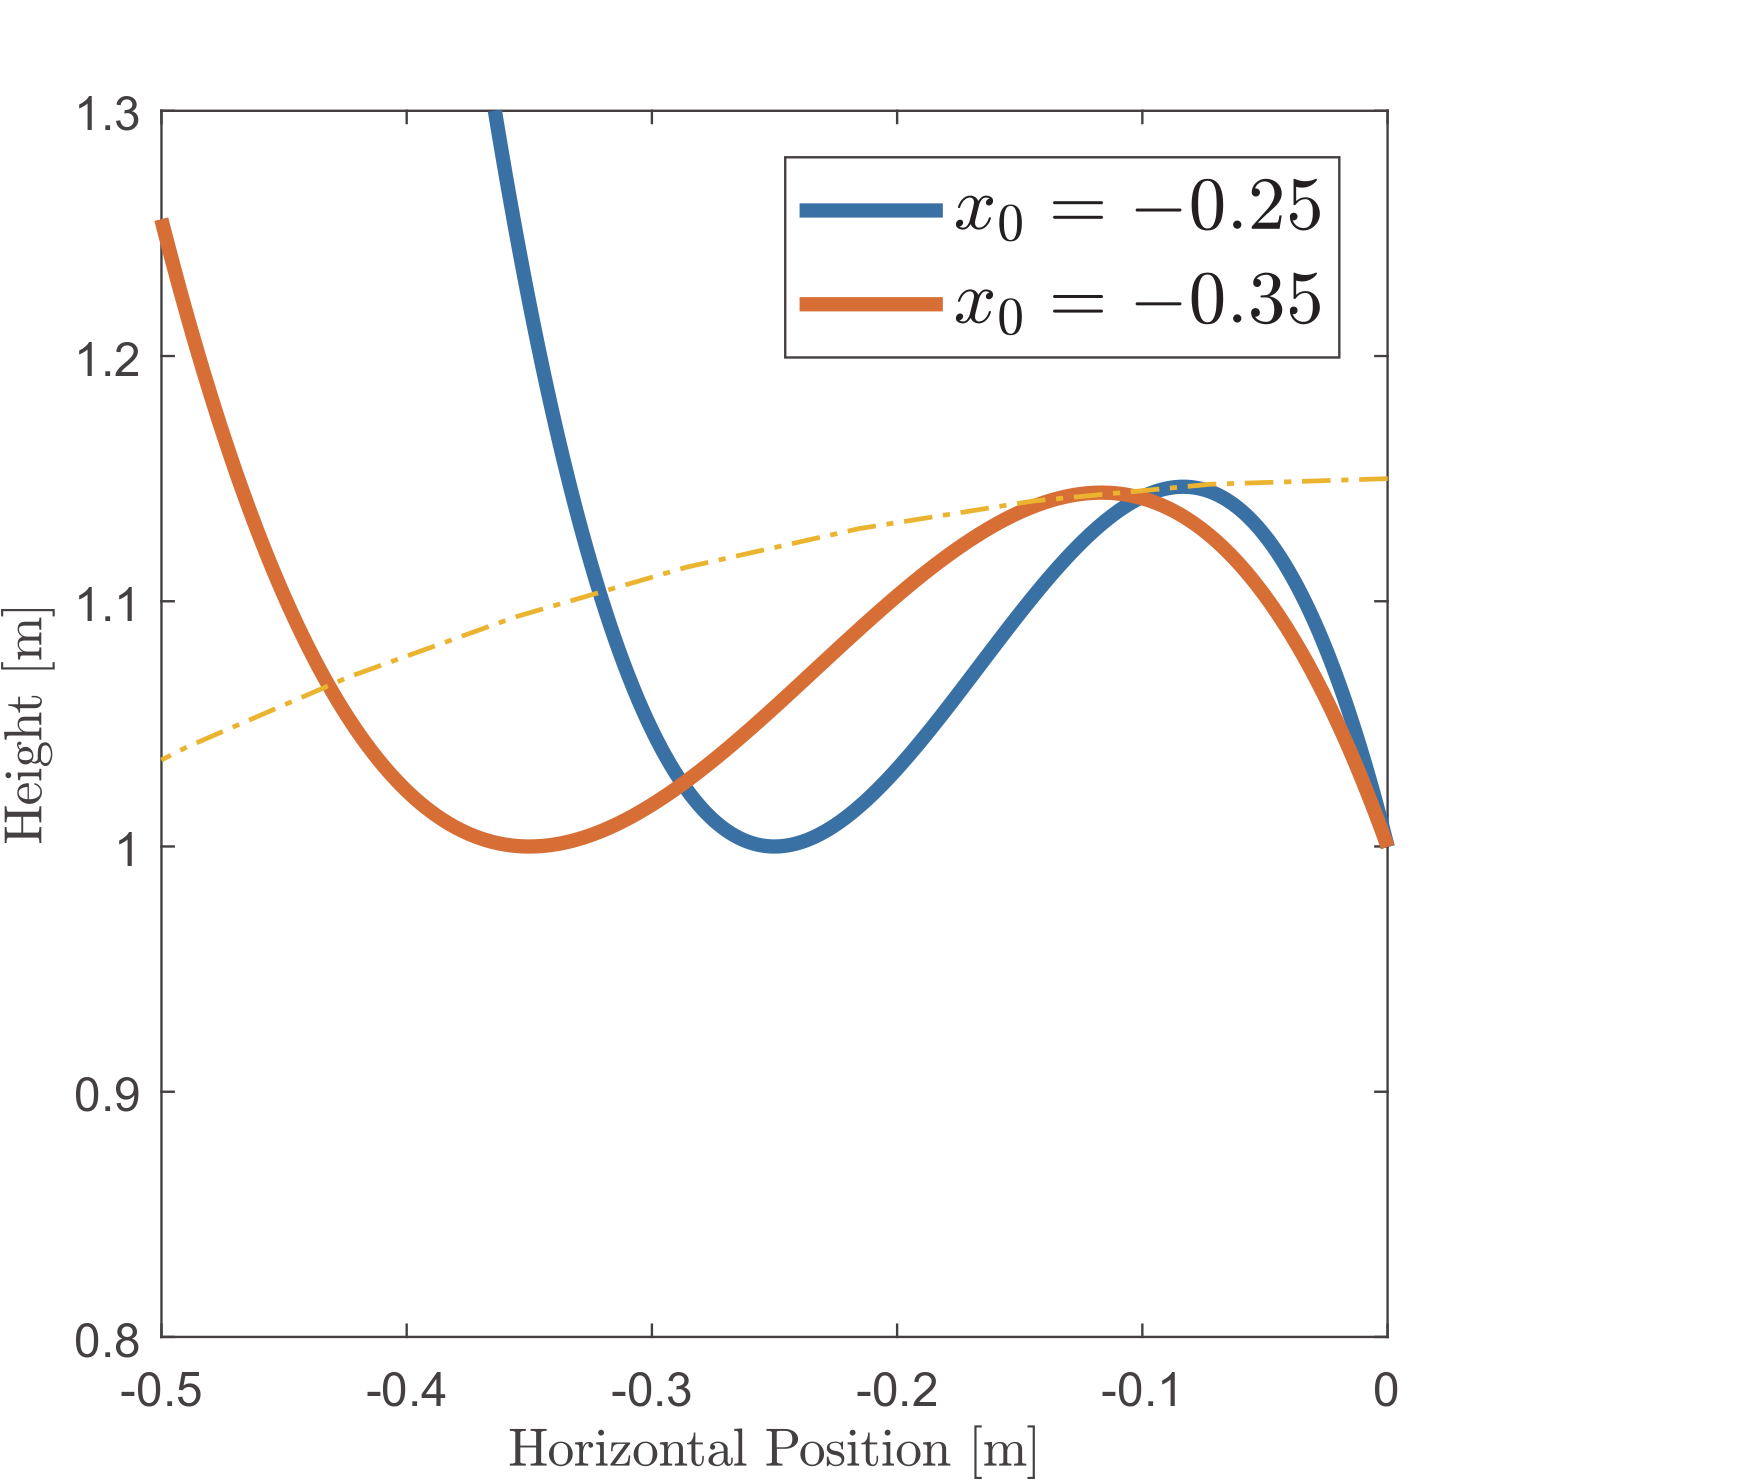
\includegraphics[width=0.6\textwidth]{STYLESTUFF/polynomialLengthViz.png}
\caption{Resulting polynomials as output from Algorithm \ref{alg:ll} with two different initial values under the final height constraint $z_f=1.0$. Other initial conditions are $\dot{x}_0=1.4$, $z_0=1.0$ and $\dot{z}_0=0$. Blue plot: $\dot{x}_f=1.107$, red plot: $\dot{x}_f=0.724$, $l_{max}=1.15$. }
\label{fig:pollength}
\end{figure}
% discussion
\section{Discussion}
The proposed algorithms can find a trajectory that gives knowledge of the estimated system state of a \ac{2D} point-foot, point-mass model until the $x$-coordinate of the point-foot. To the method of \cite{koolen2016balance}, a constraint is added on the maximum height, a maximum leg length constraint and the possibility is proposed to exchange the final height constraint with a final gradient constraint. Remarkable is that the final gradient constraint gives a higher final velocity $\dot{x}_f$ compared to the default height constraint in \figref{fig:polheight}. This is caused by the polynomial shapes, as the blue plot, under constraint $z_f$, has a steeper gradient in the first part of the trajectory after $x_0$. This is the crucial part in the trajectory for a acceleration or deceleration action in $x$-direction, as can be seen in for example Equation \eqref{eq:dynamicsprattstyle}. \\
One of the algorithms can be used in \ac{MPC}, however, it lacks a lot of properties important for application on humanoid robot as Atlas for example:
\begin{itemize}
	\item The method is only suited for a \ac{2D} control strategy.
	\item The resulting trajectory is limited by the shape of a cubic polynomial.
	\item The model is point-mass, point-foot and does not take the control options of feet or a body into account.
	\item The method is analytic and does not calculate for the next controller tick.
	\item Only a maximum height constraint is considered.
\end{itemize}
